\documentclass[conference]{IEEEtran}
\usepackage[T1]{fontenc}
\usepackage{cite}
\usepackage{amsmath,amssymb,amsfonts}
\usepackage{algorithmic}
\usepackage{graphicx}
\usepackage{textcomp}
\usepackage{xcolor}
\usepackage{booktabs}
\usepackage{multirow}
\usepackage{url}
\usepackage{tikz}
\usetikzlibrary{positioning,arrows.meta,fit,backgrounds,calc}
\usepackage{pdfpages}
% Clickable references, citations and URLs; must be loaded last.
\usepackage[hidelinks]{hyperref}


% Marks text that still needs the author's attention; delete before submitting.
\newcommand{\todo}[1]{\textcolor{red}{[TODO: #1]}}

\begin{document}

\title{Closing the Gap: Photogrammetry-Based Simulation for Sim-to-Real Transfer of
Reinforcement Learning Navigation on the Pepper Robot}

\author{\IEEEauthorblockN{Jaishil Patel - 2602867}
\IEEEauthorblockA{\textit{School of Computer Science} \\
\textit{University of the Witwatersrand}\\
Johannesburg, South Africa}
\and
\IEEEauthorblockN{Pravesh Ranchod}
\IEEEauthorblockA{\textit{School of Computer Science} \\
\textit{University of the Witwatersrand}\\
Johannesburg, South Africa}
\and
\IEEEauthorblockN{Branden Ingram}
\IEEEauthorblockA{\textit{School of Computer Science} \\
\textit{University of the Witwatersrand}\\
Johannesburg, South Africa}
}

\maketitle

\begin{abstract}
Reinforcement learning can produce navigation policies in simulation, but these policies often fail
on real robots because the simulator differs from reality. This study asks whether building the
simulator from a photogrammetric scan of the deployment room narrows this sim-to-real gap for the
Pepper humanoid robot. A real room was scanned with a tablet to create a photogrammetric simulator,
and a standard simulator of the same room was built by hand from tape measurements, so that the
source of the geometry was the only difference between them. Depth-based navigation policies were
trained in each with Soft Actor-Critic under identical domain randomisation and deployed without
further training on the physical Pepper. On the real robot, the photogrammetry policy's success rate
fell 8 percentage points below its simulated value, against 37 for the standard policy, suggesting
better transfer. It also achieved odometry-estimated success on 9 of 20 real routes against 6,
although this difference was not significant. Failures occurred in the narrow gap between the couch
and the bag, where the robot's built-in collision protection stopped it. For the two policies
tested, the results suggest that a reconstructed room yields a simulator whose results transfer more
faithfully to the real robot, while modelling the robot's own behaviour remains necessary.
\end{abstract}

\begin{IEEEkeywords}
Sim-to-Real, Photogrammetry, Reinforcement Learning, Soft Actor-Critic, Pepper Robot, GitHub: \url{https://github.com/Jaishil-Patel/ResearchCode}
\end{IEEEkeywords}

\section{Introduction}\label{sec:introduction}
Reinforcement learning (RL) lets a robot learn navigation by trial and error, but training on a
real robot is slow, costly and unsafe \cite{sutton2018rl, zhao2020sim}. Policies are therefore
trained in simulation, where they often fail once moved to the real robot because the simulator
differs from reality. This is known as the sim-to-real gap \cite{zhao2020sim,
peng2018dynamics}. It can be narrowed in two ways: by making the simulator a closer copy of
reality, or by making the policy robust to the differences that remain, for example with domain
randomisation \cite{tobin2017domain, peng2018dynamics}.

This report tests the first approach on the Pepper robot, while applying the second equally in both
simulators, whose hardware is too fragile for training on the robot itself and for which no open
simulator yet supports RL navigation \cite{sekkat2024pepper}. A real room was scanned with a tablet
and turned into a photogrammetric simulator. A second, standard simulator of the same room was built
by hand from tape measurements. Navigation policies were trained with Soft Actor-Critic (SAC) under
the same domain randomisation in each simulator and then deployed, without further training, on the
physical Pepper over the same 20 routes. Because the source of the room's geometry is the only
difference between the two, the comparison isolates the effect of the reconstruction, including its
scanning artefacts.

Using odometry-estimated success on the real robot, the photogrammetry policy showed a smaller
performance drop from simulation to reality than the standard policy, and it also reached the goal
more often, although that difference was not statistically significant. Real-robot failures for both
policies happened at the same two obstacles, where the robot's built-in collision protection stopped
it.

\section{Research Question and Hypothesis}\label{sec:rq}
\textbf{Problem.} Earlier work has shown that grounding a simulator in the real scene can improve
transfer \cite{liu2020rsr, chhablani2025embodiedsplat}, but it has not isolated the contribution
of the reconstruction itself.

\textbf{Research question.} Does training Pepper in a photogrammetry-based simulation of a room
improve its real-world navigation and reduce the sim-to-real gap, compared with a standard
simulation of the same room built by hand?

\textbf{Hypothesis.} Compared with a policy trained in the same way with SAC under domain
randomisation in a standard simulation of the room, a policy trained in a photogrammetric
reconstruction of that room will show (H1) a smaller sim-to-real gap and (H2) a higher
real-world success rate.

\section{Background}\label{sec:background}

\subsection{Reinforcement Learning and Soft Actor-Critic}
Reinforcement learning (RL) models sequential decision-making as a Markov Decision Process
(MDP): at each step the agent observes a state, takes an action, and receives a reward, and it
learns a policy that maximises the expected discounted sum of future rewards
\cite{sutton2018rl}. In mobile-robot navigation, the state usually combines a depth image with
the position of the goal relative to the robot, and the action is a continuous linear and
angular velocity \cite{chaffre2020sim}.

Soft Actor-Critic (SAC) \cite{haarnoja2018sac} is the algorithm used in this study. Besides
maximising reward, it rewards the policy for staying random by adding an entropy term to the
objective:
\begin{equation}
J(\pi)=\sum_{t=0}^{T}\mathbb{E}_{(s_t,a_t)\sim\rho_\pi}\big[r(s_t,a_t)+\alpha\,\mathcal{H}(\pi(\cdot\mid s_t))\big],
\label{eq:sac}
\end{equation}
where $\mathcal{H}$ is the entropy of the policy and the temperature $\alpha$ sets how much
exploration is valued relative to reward. A policy that does not commit too early to one way of
solving the task is less likely to overfit to the simulator. SAC is off-policy: it stores past
experience in a replay buffer and reuses it many times, learns two critics with slowly updated
target copies to avoid overestimating values, and tunes $\alpha$ automatically
\cite{haarnoja2018sac}. It suits this study because Pepper's actions are continuous, because
reusing experience matters when every simulated step runs in real time, and because it has
already been used for sim-to-real navigation \cite{chaffre2020sim}.

\subsection{The Sim-to-Real Gap and Domain Randomisation}
A policy trained in simulation often fails on the real robot, because the simulator is only an
approximation of reality \cite{zhao2020sim, peng2018dynamics}. Zhao et al.\ \cite{zhao2020sim}
divide this \emph{reality gap} into mismatches in sensing, such as camera behaviour, and in
actuation and dynamics, such as friction, mass and latency. This study uses \emph{zero-shot
transfer}: the policy runs on the real robot without any further training.

Domain randomisation varies the simulator's parameters during training, so that the range of
conditions the policy sees is wide enough to include the real world \cite{tobin2017domain}.
\emph{Dynamics randomisation} varies physical parameters such as friction and actuator delay
\cite{peng2018dynamics}, and \emph{observation randomisation} varies what the sensors report,
for example by adding noise or dropping readings. Too much randomisation can harm rather than
help real-world performance \cite{zhao2020sim}, so this study sets the ranges from measurements
of the real robot where possible (Section~\ref{sec:methodology}).

\subsection{Photogrammetry}
Photogrammetry reconstructs a textured 3D model of a real space from many overlapping
photographs, by matching the same visual features across images taken from different viewpoints
and working out their 3D positions \cite{alhamadah2024photogrammetry}. The resulting mesh can be
imported into a robot simulator. Alhamadah et al.\ \cite{alhamadah2024photogrammetry} show that
consumer devices such as smartphones can produce such models with a mean dimensional error of
about 5\%.

\subsection{The Pepper Robot and ROS~2}
Pepper is a wheeled humanoid service robot made by SoftBank Robotics and widely used in research
\cite{pandey2018pepper, sekkat2024pepper}. Its hardware is too fragile for repeated real-world
training, so simulation is needed \cite{sekkat2024pepper}. Its depth camera has a narrow field
of view, and its visual localisation drifts over distance and is sensitive to lighting
\cite{gomez2018visual}, which is why this study uses depth images and a single room. The robot is
connected to the policy through ROS~2 \cite{macenski2022ros2}, whose named data channels
(topics) are used in the same way in the Gazebo simulator \cite{koenig2004gazebo} and on the real
Pepper, so the policy's inputs and outputs stay identical across the transfer.

\section{Related Work}\label{sec:related}
In their survey of sim-to-real methods, Zhao et al.\ \cite{zhao2020sim} identify domain
randomisation as the most widely used and note that navigation has received much less attention
than manipulation. Broadly, earlier work narrows the gap from one of two directions: making the
policy robust to the mismatch that remains, or making the simulator a more faithful copy of
reality. This study combines both.

\subsection{Making the Policy Robust}
Tobin et al.\ \cite{tobin2017domain} introduce domain randomisation by varying the visual
appearance of simulated scenes, and Peng et al.\ \cite{peng2018dynamics} show that randomising
the dynamics of a simple simulator can work better than carefully building a detailed one. For
navigation, Chaffre et al.\ \cite{chaffre2020sim} train a depth-based policy with SAC and
deploy it on a real wheeled robot, doubling the real-world success rate of a naive baseline to
47\%. Their training environment, however, is a generic Gazebo world, not a model of the room
the robot is deployed in.

\subsection{Making the Simulator Realistic}
Liu et al.\ \cite{liu2020rsr} build a simplified simulation of a real scene from its semantic
layout, train a navigation policy in it and transfer it back, reaching 83\% real-world
success against 61\% for plain domain randomisation and 15\% for direct transfer. This shows
that grounding the simulator in the real scene helps, although their reconstruction is an
abstract layout rather than a realistic model. Photogrammetry can provide such a model: Guerra et
al.\ \cite{guerra2019flightgoggles} use it to render realistic camera images for drones, and
note that it is still uncommon in robot simulation, where general-purpose simulators such as
Gazebo \cite{koenig2004gazebo} are not designed for realistic rendering. Habitat
\cite{savva2019habitat} trains navigation agents in 3D-scanned indoor scenes and evaluates them
with the SPL metric of Anderson et al.\ \cite{anderson2018evaluation}, also used in this study.
More recent work reconstructs real scenes with neural radiance fields or Gaussian splatting and
trains policies inside them \cite{byravan2022nerf2real, shen2024driveenv,
chhablani2025embodiedsplat}. Closest to this study, Chhablani et al.\
\cite{chhablani2025embodiedsplat} reconstruct scenes captured with a mobile phone, train
navigation agents in them and report a strong correlation between simulated and real
performance, although for a different robot and reconstruction method.

What these studies do not isolate is the contribution of the reconstruction itself. They
compare a realistic simulator against domain randomisation or against no simulator, not against
a simulator of the \emph{same} room built by hand to the same measurements. This study makes
that comparison.

\subsection{Work on Pepper}
G\'{o}mez et al.\ \cite{gomez2018visual} build a visual navigation system for Pepper but report
drift and sensitivity to lighting. Sekkat et al.\ \cite{sekkat2024pepper} find existing Pepper
simulators to be of low fidelity, closed-source and tied to the outdated ROS~1, and build an open
ROS~2 digital twin, leaving learning-based control as future work. To our knowledge, no study has
trained an RL navigation policy for Pepper in a photogrammetric reconstruction of its environment
and tested whether the reconstruction improves transfer to the real robot.

\section{Methodology}\label{sec:methodology}

\subsection{Overview}
This section describes how the experiment was built and run. The design follows one rule: the
two simulated environments may differ only in where their geometry comes from. Everything else,
including the robot model, physics settings, task, reward, randomisation, learning algorithm and
route set, is shared. The photogrammetry world is the method under test; the standard world,
built by hand from tape measurements, is the baseline it is compared against.
Fig.~\ref{fig:pipeline} shows the full pipeline, which has five stages:
\begin{enumerate}
\item Capturing the real room with photogrammetry and checking the model against tape measurements.
\item Building two simulated versions of the room: the photogrammetric mesh, and a standard model
made of simple shapes built from the same tape measurements.
\item Integrating Pepper into the simulator and calibrating it against the real robot.
\item Training navigation policies with SAC under domain randomisation in each world.
\item Deploying one policy from each world on the physical Pepper and comparing the results.
\end{enumerate}

\begin{figure}[t]
\centering
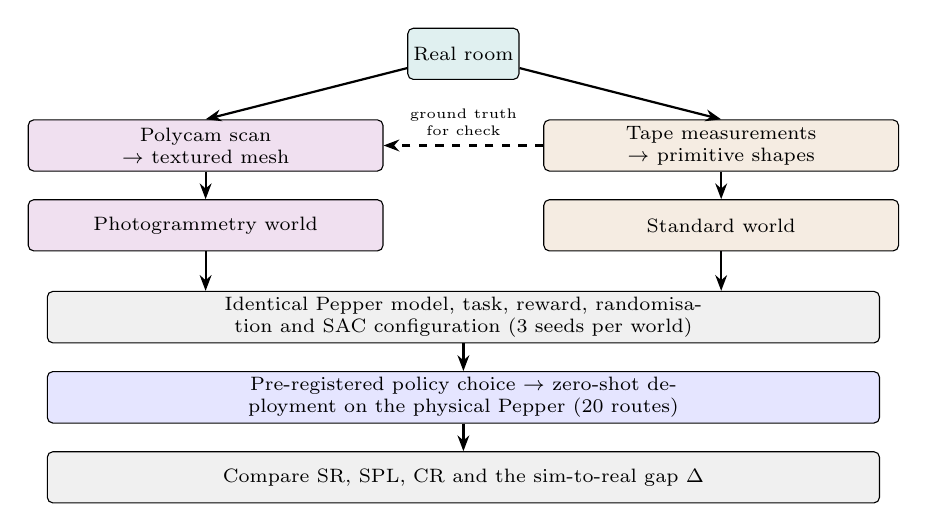
\begin{tikzpicture}[
  node distance=3.5mm and 3mm,
  box/.style={draw, rounded corners=2pt, align=center, font=\scriptsize,
              minimum height=6.5mm, inner sep=2pt},
  photo/.style={box, fill=violet!12},
  std/.style={box, fill=brown!15},
  shared/.style={box, fill=gray!12, text width=0.86\columnwidth},
  real/.style={box, fill=blue!10, text width=0.86\columnwidth},
  arr/.style={-{Stealth[length=2mm]}, thick}]
\node[box, fill=teal!12] (room) {Real room};
\node[photo, below=5mm of room, xshift=-0.27\columnwidth, text width=0.36\columnwidth] (scan)
  {Polycam scan\\ $\rightarrow$ textured mesh};
\node[std, below=5mm of room, xshift=0.27\columnwidth, text width=0.36\columnwidth] (tape)
  {Tape measurements\\ $\rightarrow$ primitive shapes};
\node[photo, below=of scan, text width=0.36\columnwidth] (pw) {Photogrammetry world};
\node[std, below=of tape, text width=0.36\columnwidth] (sw) {Standard world};
\node[shared, below=5mm of $(pw.south)!0.5!(sw.south)$] (train)
  {Identical Pepper model, task, reward, randomisation and SAC configuration (3 seeds per world)};
\node[real, below=of train] (deploy)
  {Pre-registered policy choice $\rightarrow$ zero-shot deployment on the physical Pepper (20 routes)};
\node[shared, below=of deploy] (eval) {Compare SR, SPL, CR and the sim-to-real gap $\Delta$};
\draw[arr] (room) -- (scan.north);
\draw[arr] (room) -- (tape.north);
\draw[arr, dashed] (tape.west) -- node[above, font=\tiny, align=center] {ground truth\\for check} (scan.east);
\draw[arr] (scan) -- (pw);
\draw[arr] (tape) -- (sw);
\draw[arr] (pw.south) -- (pw.south |- train.north);
\draw[arr] (sw.south) -- (sw.south |- train.north);
\draw[arr] (train) -- (deploy);
\draw[arr] (deploy) -- (eval);
\end{tikzpicture}
\caption{The experimental pipeline. The two branches (purple: photogrammetry (method), brown:
standard (baseline)) differ only in the source of the room geometry; every later stage is shared.}
\label{fig:pipeline}
\end{figure}

\subsection{The Photogrammetry Branch}
The target room is a $5.5 \times 4.2$\,m storage room containing a couch, two chairs, a shelf, three
large boxes, a bag, a green pole and a red pole that serves as the navigation goal
(Fig.~\ref{fig:layout}). It was captured with the Polycam application in photo mode on an iPad Pro
11-inch (2nd generation). Over a 10--30 minute session, overlapping photographs were taken while
walking around the room, at several heights, and around each piece of furniture so that it was
seen from all sides. The room lights were on, nothing was moved during the capture, and no
people were in the room. Polycam then processed the photographs into a textured 3D mesh using
photogrammetry (Section~\ref{sec:background}), which was exported as a GLB file. The mesh was
already at metric scale, so no scale correction was applied; the accuracy gate below confirms
this.

A custom import script (\texttt{mesh\_import.py}) converted the mesh into a simulator model in
a repeatable way. It aligned the room with the simulator axes, placed the origin at
the floor corner, smoothed scanning noise with a light Taubin filter, and reduced the mesh to
50{,}000 faces (using Blender) so the physics engine could run it in real time. Every transform was saved to a
manifest file so the import can be reproduced exactly.

Before training, the model had to pass an accuracy gate. Ten room dimensions ($K=10$) were measured
with a tape measure, including room length, width and height, and the heights of the furniture, and
the same dimensions were measured on the mesh. The mean absolute percentage error was
\begin{equation}
\bar{e} = \frac{1}{K}\sum_{k=1}^{K}\frac{|m_k-\hat{m}_k|}{m_k}\times 100\%,
\label{eq:gate}
\end{equation}
where $m_k$ is the tape measurement and $\hat{m}_k$ the mesh measurement. The threshold was the
4.97\% reported for consumer-grade photogrammetry by Alhamadah et al.\
\cite{alhamadah2024photogrammetry}. The reconstruction achieved $\bar{e}=2.12\%$. The largest
errors were on soft objects (couch height 6.85\%, bag height 5.70\%), and the room dimensions
were within about 1\%.

Two problems appeared once Pepper drove on the scanned floor. First, the floor was tilted by
$1.78^\circ$, so the mesh was levelled to $0.01^\circ$. Second, small bumps in the scanned floor
caught Pepper's wheels and left the robot stuck. To fix this, only the \emph{collision} mesh was
flattened below 0.12\,m (high enough to remove the bumps in the scanned floor, but lower than
any real object in the room). The visual mesh, which the depth camera sees, was not changed, and the
accuracy gate still gave 2.12\%.

\subsection{The Standard Branch}
The standard world is the baseline an engineer would build by hand. It was generated from the same
tape measurements as the gate: walls, a flat floor, and one box-shaped primitive per furniture item,
each with its measured size and position. What it lacks is the irregular surface detail that
photogrammetry recovers, such as the shape of the couch, the open shelf compartments and the bag.
Both world files are generated from a single template, and an automatic check confirms that the only
difference between them is which room model is included. Fig.~\ref{fig:worlds} compares the two
worlds.

\begin{figure}[t]
\centering
\IfFileExists{figures/worlds.png}{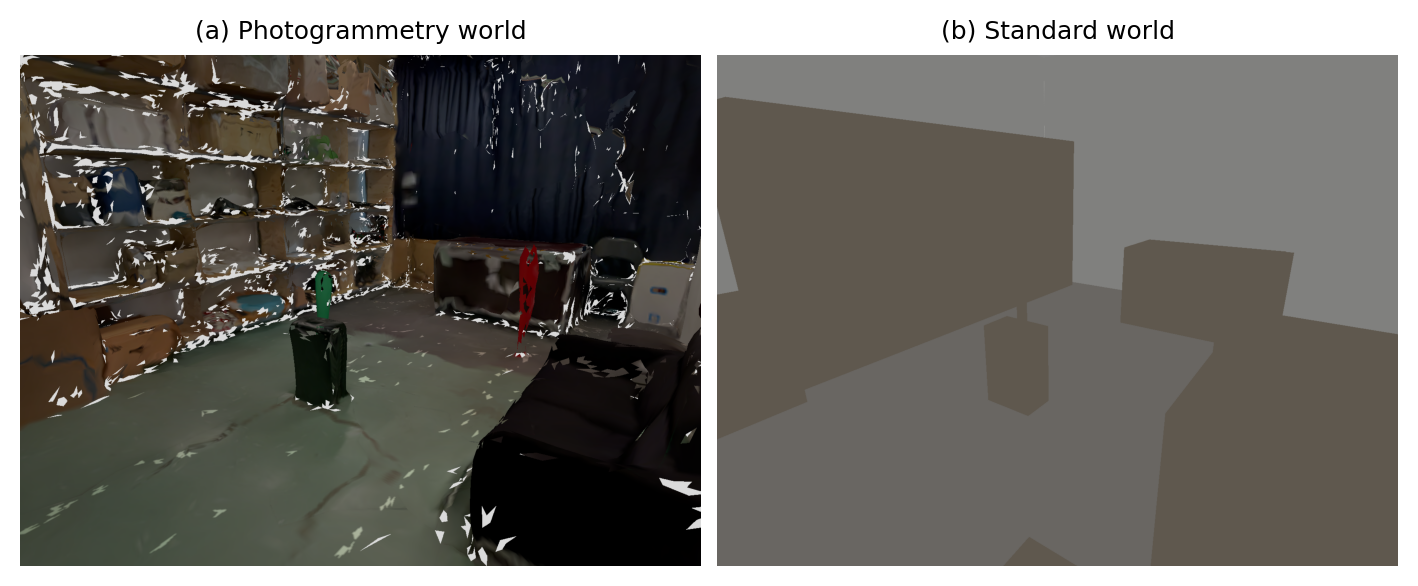
\includegraphics[width=\columnwidth]{figures/worlds}}%
{\fbox{\parbox[c][3cm][c]{0.9\columnwidth}{\centering\todo{figures/worlds.png: photogrammetry
world (left) and standard world (right), same viewpoint}}}}
\caption{The same view of the photogrammetry world (left) and the standard world (right). The
white flecks are texture artefacts from mesh decimation; they affect colour only, and the policy
observes depth.}
\label{fig:worlds}
\end{figure}

\subsection{Pepper in Simulation}
Pepper was simulated in Ignition Gazebo (Fortress) with ROS~2 Humble, using the DART physics engine
with Bullet collision detection and a 5\,ms step, and an open-source Pepper description that was
ported to ROS~2 Humble for this project. The policy uses only ROS 2 topics that also exist on the
real robot: the depth image from the head camera, the odometry of the base, and velocity commands to
the base. This means the same code drives both the simulated and the physical robot. The head was
fixed at a pitch of 0.45\,rad (looking down) in both simulation and reality. At Pepper's default
upward head angle, low obstacles such as the bag and the boxes leave the depth image when they are
still about 3\,m away.

Collisions are detected with contact sensors on eight links (base, torso, upper arms, forearms
and hands), and a tilt of more than $20^\circ$ is also treated as a collision (normal driving
never tilts Pepper by more than about $6^\circ$, so a larger tilt means the robot is falling
over). On the real robot,
the three base bumpers provide the same collision signal.

The simulated base was then calibrated against the real robot. The same set of velocity commands
(straight, reverse, spins and arcs) was sent to both, and their responses were compared. The real
robot reached its commanded speeds to within about 5\%, but responded with a median delay of 0.85\,s
through the full communication chain, while the simulated base responded almost instantly. The
simulator was therefore given a four-step (0.8\,s) command delay and acceleration limits fitted
to the real measurements.

\subsection{The Navigation Task}
The task is point-to-point navigation. Pepper starts at a pose in the room and must reach the red
goal pole, at $(3.75, 1.10)$\,m, without colliding. It is modelled as an MDP as follows.

\textbf{Observation.} At each step the policy receives:
\begin{itemize}
\item a $64\times48$ depth image, limited to 0.4--8.0\,m (the range of the simulated camera; the
real camera's readings were cut to the same range, and anything outside it, including missing
readings, is treated as far away);
\item the goal relative to the robot, as $(d, \sin\theta, \cos\theta)$, where $d$ is the distance
and $\theta$ the bearing;
\item the last six actions. Because commands take effect about 0.8\,s after they are sent, this
history tells the policy what it has already asked the robot to do.
\end{itemize}

\textbf{Action.} A continuous linear velocity $v\in[-0.10, 0.30]$\,m/s and angular velocity
$\omega\in[-0.90, 0.90]$\,rad/s, sent at 5\,Hz.

\textbf{Reward.} Each step's reward is
\begin{equation}
r_t = -0.05 + 20\,(d_{t-1}-d_t) - 0.02\,|\omega_t|,
\label{eq:reward}
\end{equation}
which consists of a small time penalty, a reward for every metre of progress towards the goal,
and a small penalty for turning. In addition, $+100$ is given for reaching the goal and $-100$ for
a collision.

\textbf{Episode end.} An episode ends when Pepper's base centre is within 0.6\,m of the goal
(success), when it collides or tips over, or after 120\,s.

\textbf{Starts and routes.} During training, each episode starts at a random collision-free position
with a random heading, so that the policy cannot memorise the validation starts. For evaluation, a
fixed set of 20 validation routes was generated (Fig.~\ref{fig:layout}). The shortest feasible path
length $\ell^*$ of each route was planned on the tape-measured map with obstacles enlarged by
0.32\,m to allow for Pepper's body. The same 20 routes are used for both branches, in simulation
and on the real robot. They were also used to choose which seed to deploy, so they are validation
routes rather than an untouched test set. Before the final training runs, short development runs
on them led to corrections of the simulation: the scanned floor was levelled, contact sensors were
added, the camera was tilted down to see low obstacles, and the goal tolerance and tip-over rule
were set. The action history and the latency, depth-noise and frame-rate randomisation were
added or set from measurements of the real robot rather than from route results. The reward,
network and SAC hyperparameters were set before the final training runs and not changed after.
The evaluations every 25{,}000 steps were used only for monitoring; the deployed policies are the
final ones at 300{,}000 steps.

\begin{figure}[t]
\centering
\IfFileExists{figures/layout.pdf}{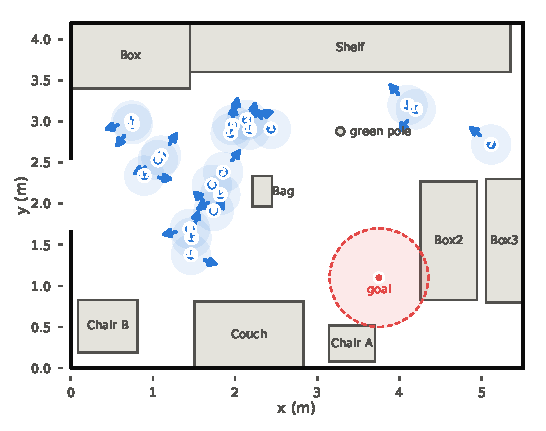
\includegraphics[width=\columnwidth]{figures/layout}}%
{\fbox{\parbox[c][4cm][c]{0.9\columnwidth}{\centering\todo{figures/layout.pdf: top-down room
plan with the 20 route starts and the goal zone}}}}
\caption{Top-down plan of the room with the 20 validation route starts (blue, arrows show the starting
heading) and the 0.6\,m goal zone around the red pole.}
\label{fig:layout}
\end{figure}

\subsection{Domain Randomisation}
Both branches were trained with the same randomisation (Table~\ref{tab:randomisation}). Each
parameter is sampled at the start of every episode and held fixed for that episode, following
Peng et al.\ \cite{peng2018dynamics}. Where possible, the ranges were set from measurements of the
real robot rather than chosen by hand. The command delay is varied around the measured 0.8\,s. The
depth noise matches the 5.5\,mm median frame-to-frame noise measured on the real camera. The
dropout patches imitate a full-height band with no depth readings that a window produced in the
real camera's image. The depth frame rate is varied because the real camera delivered only
1.9--3 frames per second over Wi-Fi during calibration, well below the 5\,Hz control rate. When
no new frame arrives, the policy receives the previous one again.

\begin{table}[t]
\caption{Randomisation applied during training, identical for both branches}
\label{tab:randomisation}
\centering
\footnotesize
\begin{tabular}{@{}llr@{}}
\toprule
Group & Parameter & Range \\
\midrule
\multirow{5}{*}{Command} & Linear / angular velocity scale & $\times$0.8--1.2 \\
 & Linear velocity noise (std) & 0.02\,m/s \\
 & Angular velocity noise (std) & 0.05\,rad/s \\
 & Command delay (around 4 steps) & $\pm$2 steps \\
 & Wheel slip probability & 0--0.05 \\
\midrule
\multirow{3}{*}{Depth} & Per-pixel noise (std) & 0.01\,m \\
 & Pixel and patch dropout & 0--15\% \\
 & Frame rate (log-uniform) & 1.5--15\,Hz \\
\midrule
Surface & Floor friction coefficient $\mu$ & 0.6--1.2 \\
\bottomrule
\end{tabular}
\end{table}

\subsection{Training with Soft Actor-Critic}
The policies were trained with the SAC implementation in Stable-Baselines3
\cite{haarnoja2018sac}, \cite{raffin2021sb3}. A small convolutional network, the
NatureCNN encoder from DQN \cite{mnih2015dqn}, encodes the depth image into 128 features, which are joined with the goal vector and action history and passed to
two fully connected layers of 256 units. The hyperparameters were the same for every run:
\begin{itemize}
\item learning rate $3\times10^{-4}$, discount $\gamma=0.99$, target update $\tau=0.005$;
\item replay buffer of 100{,}000 transitions, batch size 256, 2{,}000 warm-up steps;
\item one gradient step per environment step, and automatic entropy tuning;
\item 300{,}000 environment steps per run.
\end{itemize}

Three runs (seeds 0, 1 and 2) were trained per branch, six in total. One run takes 20--33 hours
of wall-clock time, so the runs were executed in parallel on the Wits mathematical sciences
cluster inside an Apptainer container. Training saved checkpoints every 25{,}000 steps and
resumed automatically when the simulator stalled. Every 25{,}000 steps, each run was evaluated
once on the 20 routes.

After training, each final policy was evaluated in its own world over five independent sessions
of the 20 routes. Several sessions are needed because the simulator runs in real time rather
than in fixed steps, so repeated runs of the same policy do not give identical results. Before
any real-robot run, a rule was fixed for choosing which policy from each branch to deploy: the
seed with the highest simulated SR, with ties broken by SPL. This selected standard seed~1 and
photogrammetry seed~0.

\subsection{Deployment on the Real Pepper}
The policies were deployed zero-shot, with no fine-tuning on the real robot. Pepper's software
(NAOqi 2.5) supports only Python 2.7 for its Python SDK, so a small Python~2 program on the laptop
talks to the robot over the network, and a ROS~2 bridge node republishes its data under the same
topic names as the simulator. The policy therefore runs unchanged. The depth image ($160\times120$
requested at 5\,Hz), odometry, bumper states and velocity commands all pass through this link. As a
safety measure, the robot stops if no command arrives for 1.5\,s, and the emergency stop button was
always within reach. For safety, NAOqi's built-in collision protection, which slows or stops the
base near obstacles, was kept on for all real trials.

The 20 routes were taped onto the floor of the real room. For each route, the operator placed Pepper
on the taped start, and its odometry was reset to that known pose. The policy then ran until
success, collision or 120\,s. Contacts that the base bumpers cannot detect, such as an arm brushing
furniture, were noted by the operator. The evaluation took place over two days (routes r000--r010
and r011--r019), and the order of the two policies was swapped on the second day.

\subsection{Evaluation Metrics}
Four metrics are used. Over the $N=20$ routes, the \emph{success rate} is
$\mathrm{SR}=\frac{1}{N}\sum_i S_i$, where $S_i=1$ if route $i$ ended within 0.6\,m of the goal with
no collision before the time limit, and 0 otherwise. On the real robot, no external tracking was
available, so whether a route succeeded and the distance travelled both come from odometry, reset at
the taped start of each route. We call this odometry-estimated success. Real-robot SR and SPL are
therefore odometry-estimated, and the sim-to-real gap compares them with simulated values computed
from the true pose.

The \emph{success weighted by path length} \cite{anderson2018evaluation} also rewards efficient
paths:
\begin{equation}
\mathrm{SPL}=\frac{1}{N}\sum_{i=1}^{N} S_i\,\frac{\ell^*_i}{\max(\ell_i,\ell^*_i)},
\label{eq:spl}
\end{equation}
where $\ell_i$ is the distance actually travelled. The \emph{collision rate} CR is the number of
collisions per metre travelled. The \emph{sim-to-real gap} for a metric $M$ is
\begin{equation}
\Delta M = M_{\text{sim}} - M_{\text{real}},
\label{eq:gap}
\end{equation}
computed separately for each branch. A smaller $\Delta$ means the simulator predicted real
performance better.

The main comparison is between branches: photogrammetry is considered better if
$\Delta_{\text{photo}}$ is smaller than $\Delta_{\text{std}}$. This is tested per route with the
Wilcoxon signed-rank test ($\alpha=0.05$) on the paired differences
$\Delta_{\text{photo},i}-\Delta_{\text{std},i}$, where a route's gap is its mean simulated outcome
over the five sessions minus its real outcome. Real-robot performance of the two policies is also
compared directly. Both tests pair each route with itself, because both branches use the same
20 routes. The same paired test checks whether each branch's own gap is larger than zero. 95\%
confidence intervals for the real-robot SR use the Wilson score interval.

\section{Results and Discussion}\label{sec:results}
This section first reports how the policies performed in simulation and on the real robot.
It then compares the sim-to-real gap of the two branches, which is the main question of this
study, and finally looks at why the real robot failed on most routes.

\subsection{Simulation Results}
Table~\ref{tab:sim} shows the final simulated performance of all six policies, each evaluated over
five sessions of the 20 routes. The standard policies performed better in simulation, with a mean SR
of 0.58 against 0.42 for photogrammetry. The seeds also varied considerably: standard seed~2 reached
only 0.39, while seeds 0 and 1 both reached 0.67. A likely reason for the lower photogrammetry
scores is that its world is harder to navigate: the scanned obstacles have irregular shapes, and the
mesh has small cracks that leave gaps in the depth image (Fig.~\ref{fig:worlds}; appendix,
Fig.~\ref{fig:depth}), whereas the standard world contains only clean boxes. The training curves are
given in the appendix (Fig.~\ref{fig:training}). Following the rule fixed before the real trials,
standard seed~1 and photogrammetry seed~0 were deployed on the robot.

\begin{table}[t]
\caption{Final simulated performance (mean $\pm$ standard deviation over five sessions of 20
routes). $^\ast$ marks the policy deployed on the real robot.}
\label{tab:sim}
\centering
\footnotesize
\begin{tabular}{@{}llccc@{}}
\toprule
Branch & Seed & SR & SPL & CR (per m) \\
\midrule
\multirow{4}{*}{Standard}
 & 0 & 0.67$\pm$0.06 & 0.54$\pm$0.05 & 0.09 \\
 & 1$^\ast$ & 0.67$\pm$0.08 & 0.59$\pm$0.06 & 0.17 \\
 & 2 & 0.39$\pm$0.07 & 0.37$\pm$0.06 & 0.46 \\
 & Mean & 0.58 & 0.50 & 0.24 \\
\midrule
\multirow{4}{*}{Photogrammetry}
 & 0$^\ast$ & 0.53$\pm$0.08 & 0.48$\pm$0.07 & 0.30 \\
 & 1 & 0.44$\pm$0.15 & 0.38$\pm$0.12 & 0.36 \\
 & 2 & 0.29$\pm$0.09 & 0.27$\pm$0.08 & 0.59 \\
 & Mean & 0.42 & 0.38 & 0.42 \\
\bottomrule
\end{tabular}
\end{table}

\subsection{Real-Robot Results}
Both deployed policies performed worse on the real robot than in simulation (Table~\ref{tab:real}).
By odometry-estimated success, the photogrammetry policy succeeded on 9 of 20 routes (SR
0.45) and the standard policy on 6 of 20 (SR 0.30). The
photogrammetry policy therefore did better on the real robot, but the 95\% confidence intervals
overlap, and the paired per-route comparison does not show a significant difference (SR
$p=0.18$, SPL $p=0.07$).

Collisions were rarer on the real robot than in simulation (0.032 per metre for standard and 0.055
for photogrammetry). This is mainly because NAOqi's collision protection, which was kept on for
safety, slowed or stopped the base near obstacles. Instead of colliding, the robot often stopped in
front of an obstacle until the time ran out (Section~\ref{sec:results-why}).

\begin{table}[t]
\caption{The two deployed policies in simulation and on the real robot (20 routes each). Real values are odometry-estimated. $\Delta$ is simulated
minus real; $p$ is the paired per-route Wilcoxon test.}
\label{tab:real}
\centering
\footnotesize
\setlength{\tabcolsep}{4pt}
\begin{tabular}{@{}lcc@{}}
\toprule
 & Standard (seed 1) & Photogrammetry (seed 0) \\
\midrule
Sim SR / SPL & 0.67 / 0.59 & 0.53 / 0.48 \\
Real SR & 0.30 [0.15, 0.52] & 0.45 [0.26, 0.66] \\
Real SPL & 0.16 & 0.27 \\
Real CR (per m) & 0.032 & 0.055 \\
\midrule
$\Delta$SR ($p$) & 0.37 (0.009) & 0.08 (0.392) \\
$\Delta$SPL ($p$) & 0.43 (0.001) & 0.21 (0.022) \\
\midrule
\multicolumn{3}{@{}l}{Is $\Delta_{\text{photo}} < \Delta_{\text{std}}$? SR: $p=0.03$, SPL:
$p=0.01$} \\
\bottomrule
\end{tabular}
\end{table}

\begin{figure}[t]
\centering
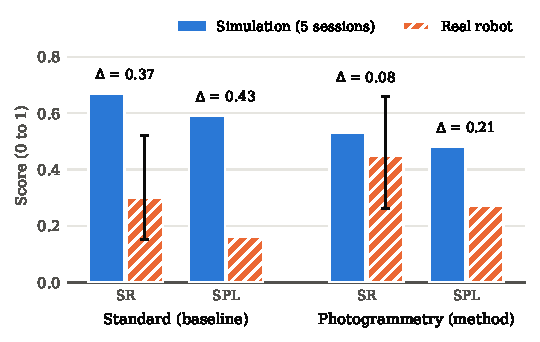
\includegraphics[width=\columnwidth]{figures/results_bars}
\caption{SR and SPL of the two deployed policies in simulation and on the real robot. Error bars on the real SR are 95\% Wilson intervals;
$\Delta$ is the sim-to-real gap.}
\label{fig:bars}
\end{figure}

\subsection{The Sim-to-Real Gap}
The photogrammetry policy lost less performance when moved to the real robot (Fig.~\ref{fig:bars}).
Its success rate fell by 8 percentage points (from 0.53 in simulation to 0.45 on the robot), while
the standard policy's fell by 37 points (from 0.67 to 0.30). Measured by SPL, which also rewards
short paths, the photogrammetry policy's drop (0.21) was about half that of the standard policy
(0.43). Comparing the two gaps route by route, the photogrammetry gap was smaller on 12 routes and
the standard gap on 3, and the difference is statistically significant ($p=0.03$ for SR, $p=0.01$
for SPL). This supports the hypothesis for the two deployed policies: the policy trained in the
photogrammetry world transferred with a smaller loss of performance. Because the test pairs routes
rather than independent training runs, it does not show that this holds across training seeds
(Section~\ref{sec:limitations}).

The smaller gap has two sources. The photogrammetry policy scored lower in simulation
(0.53 against 0.67), so its simulator gave a less optimistic prediction,
and it scored higher on the real robot (0.45 against 0.30). The standard
policy's gap was large and significant (SR $p=0.009$, SPL $p=0.001$), so its
simulator clearly over-predicted real performance. For the photogrammetry policy, only the SPL
gap was significant ($p=0.022$), while its SR gap was not ($p=0.392$): its
simulated success rate was a reasonable prediction of its real one, although it reached the goal
by less efficient paths on the real robot.

\subsection{Why the Real Robot Failed}\label{sec:results-why}
Table~\ref{tab:failures} groups every real route by how it ended, using the scored result and the
operator's notes. Two factors stand out.

\begin{table}[t]
\caption{How each real route ended (20 routes per policy)}
\label{tab:failures}
\centering
\footnotesize
\begin{tabular}{@{}lcc@{}}
\toprule
Outcome & Standard & Photogrammetry \\
\midrule
Reached the goal & 6 & 9 \\
Collided (all with the couch) & 2 & 3 \\
Stopped at the couch or bag until timeout & 5 & 5 \\
Stopped within 1\,m of the goal (near miss) & 2 & 0 \\
Barely moved ($<1$\,m) & 1 & 3 \\
Other timeout & 4 & 0 \\
\bottomrule
\end{tabular}
\end{table}

\textbf{The couch and the bag.} Many failures happened at two obstacles. The couch lies between many
of the starts and the goal, and the bag stands in the middle of the room (Fig.~\ref{fig:layout}).
Every collision was with the couch, and many more routes ended with the robot stopped in front of
the couch or the bag. In simulation, the policies reach the goal from the left of the room by
driving through the gap between the bag and the couch, passing close to the couch (appendix,
Fig.~\ref{fig:paths}). On the real robot this same gap is where most runs failed: NAOqi's collision
protection held the base back when it came close to an obstacle, while the policy kept commanding it
towards the goal. The policy had never experienced this behaviour in training, so it had not learned
to back off and try another path.

\textbf{Real-robot conditions.} The real robot also differed from the simulator in ways the
randomisation only approximated. The control loop ran at 5\,Hz over Wi-Fi with depth images at
$160\times120$, and commands took effect about 0.85\,s after they were sent. Together with the collision protection, these
conditions made the robot slower and more hesitant than in simulation, which helps explain the
many timeouts and the low SPL on the real robot.

\section{Limitations}\label{sec:limitations}
The study has several limitations that affect how far its results can be generalised:
\begin{itemize}
\item \textbf{Scale of the evaluation.} The study uses one room, 20 routes and one real-robot
session per policy, and only one trained policy from each branch is deployed. The samples are small,
the confidence intervals on the real success rates are wide, and the results may not hold in other
rooms. The 20 routes pair the two policies route by route, but they are not independent training
runs, so the $p$-values describe these two selected policies on these routes. They do not show that
photogrammetry-trained policies in general transfer better across training seeds.
\item \textbf{Seed selection.} The deployed policy in each branch is the seed with the highest
simulated SR on the same validation routes. Choosing the best of three seeds on these routes biases
its simulated SR upwards, and therefore inflates $\Delta$, for both branches.
\item \textbf{Position measurement.} No external tracking system is available. The robot's final
position comes only from odometry estimates.
\item \textbf{Robot conditions.} NAOqi's collision protection is kept on for safety and stops the
robot near obstacles, which the policies never experience in training. The robot is controlled over
Wi-Fi at 5\,Hz with a command delay of about 0.85\,s, and mass and centre of mass are not
randomised.
\item \textbf{Simulation fidelity.} The simulator runs in real time and is not deterministic, so
repeated evaluations of the same policy differ and five sessions are needed. The scanned mesh has
small cracks that leave gaps in the depth image, adding depth noise that the standard world lacks,
so the effect of the room's shape cannot be fully separated from that of these artefacts. Its
largest errors are on soft objects (up to 6.85\%). The room is static, with no people or moving
objects. Depth readings closer than 0.4\,m are treated as far away, although, with the camera 1.1\,m
above the floor, this only affects objects already touching the robot.
\end{itemize}

\section{Future Work}\label{sec:future}
Several extensions would strengthen and extend these results:
\begin{itemize}
\item \textbf{Robustness test.} A natural next step is a perturbed version of the room, with the bag
and the green pole moved and ten new routes. It would show whether the photogrammetry policy also
copes better when the room no longer matches its scan.
\item \textbf{Position tracking and more trials.} An overhead camera or motion-capture system would
remove the dependence only on odometry. More real sessions, and more than one deployed policy per
branch, would narrow the confidence intervals.
\item \textbf{Collision protection.} Many real failures happened when NAOqi's collision protection
held the robot in front of the couch or the bag. Modelling this behaviour in simulation, or training
with it, would remove the largest source of failure.
\item \textbf{Other rooms and reconstructions.} Repeating the comparison in several rooms, and with
newer reconstruction methods such as Gaussian splatting \cite{chhablani2025embodiedsplat}, would
show how general the benefit of a reconstructed simulator is.
\end{itemize}

\section{Conclusion}\label{sec:conclusion}
This study built two simulators of the same room for Pepper, one from a photogrammetric scan and
one by hand from tape measurements, trained a SAC navigation policy in each under identical domain
randomisation, and deployed both on the real robot without further training.

On H1, the photogrammetry policy has a significantly smaller sim-to-real gap: its success rate fell
by 8 percentage points from simulation to the real robot, against 37 for
the standard policy. On H2, its odometry-estimated success is 9 of 20 real routes against 6, which
points the same way but is not statistically significant. Most real failures of both policies
happened at the couch and the bag, where collision protection, unseen in training, stopped the
robot.

For the two policies tested, the results suggest that a reconstructed room transfers to the real
robot more faithfully than a hand-built one made from the same measurements. Whether this holds
across training seeds needs more than one deployed policy per branch. Photogrammetry alone is not enough, however:
transfer also depends on modelling the robot's own behaviour, such as its collision protection,
and confirming the real-world difference needs larger trials with external position tracking.


\bibliographystyle{IEEEtran}
\bibliography{refs}

\clearpage
\onecolumn
\appendix
\section{Additional Figures and Tables}\label{sec:appendix}

\begin{figure}[!h]
\centering
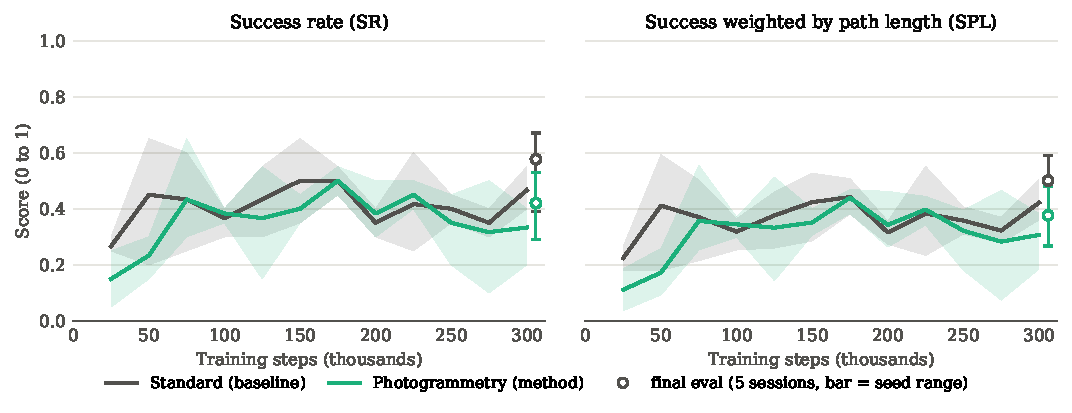
\includegraphics[width=\textwidth]{figures/training_curves}
\caption{Simulated SR (left) and SPL (right) during training, measured on the 20 routes every
25{,}000 steps (one session per point). Lines are the mean of the three seeds of each branch and
the shaded bands the range across seeds. Hollow markers at 300k are the final five-session
evaluations used in Table~\ref{tab:sim} (seed mean, bar showing the seed range). Single-session
evaluations of one seed jump by as much as 0.5 between neighbouring points, which is why the final
results use five sessions.}
\label{fig:training}
\end{figure}

\begin{figure}[!h]
\centering
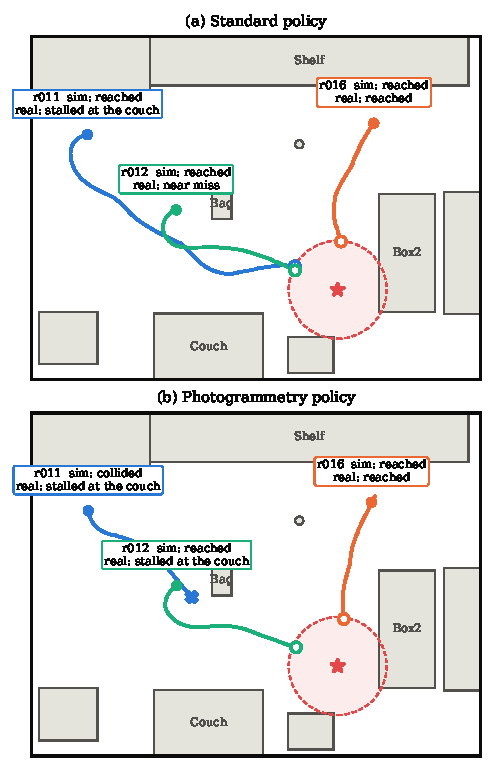
\includegraphics[width=0.42\textwidth]{figures/paths}
\caption{Simulated paths of the two deployed policies on three example routes (one rollout
each; filled dot: start, hollow circle: reached, cross: collision). The label gives the outcome
of the same route in simulation and on the real robot, whose path was not recorded.}
\label{fig:paths}
\end{figure}

\begin{figure}[!h]
\centering
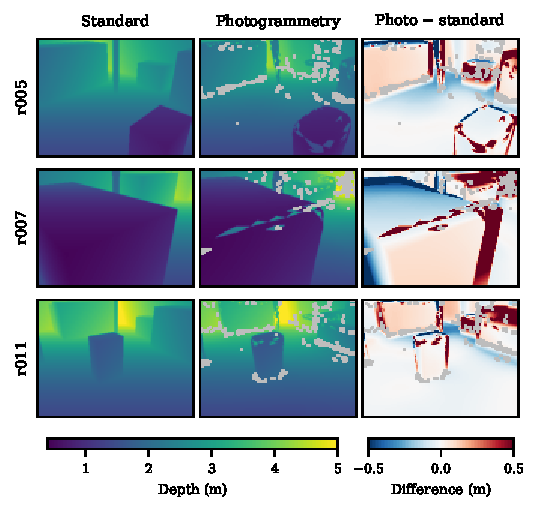
\includegraphics[width=0.42\textwidth]{figures/depth_compare}
\caption{Simulated depth images from identical poses in the two worlds: the head camera at the
start of three routes, turned to face the goal, with no robot in the scene. The right column is
photogrammetry minus standard depth. Grey pixels have no depth reading and are read by the policy
as far away; in the photogrammetry world they mostly come from small cracks in the scanned mesh.
The two worlds agree on the walls and floor, and differ mainly at the edges of objects, where the
scanned shapes replace the standard world's boxes.}
\label{fig:depth}
\end{figure}


\clearpage
% Wits Faculty of Science AI declaration -- the signed form, included as a full page.
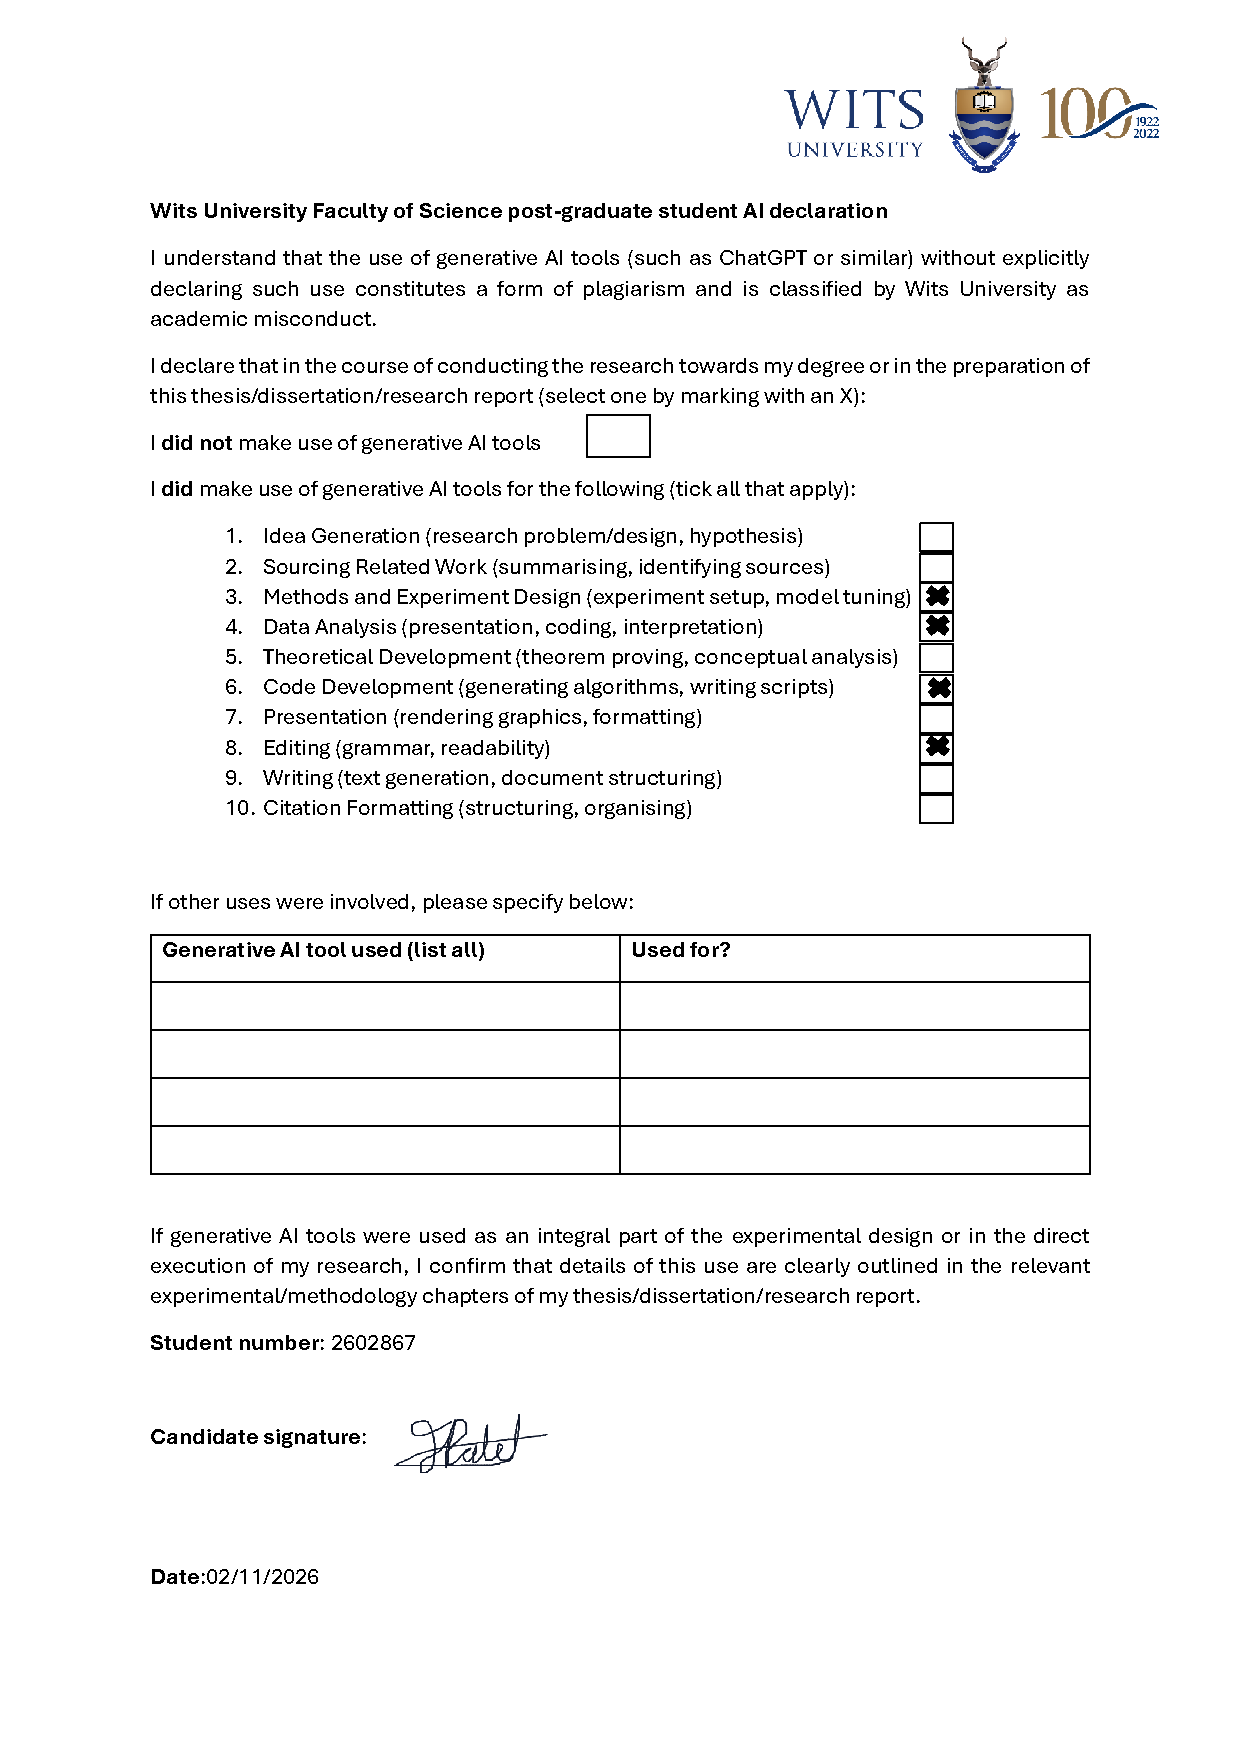
\includepdf[pages=1]{ai_declaration.pdf}


\end{document}
